\setcounter{page}{1} % Iniciar la numeración de las páginas en este punto

\section{Introducción}


\section{Antecedentes}

    \subsubsection*{A chest-based continuous cuffless blood pressure method: Estimation and evaluation using multiple body sensors \cite{bodySensor}.}

    El artículo analiza el desarrollo de un dispositivo no invasivo para la estimación de la presión arterial (PA) utilizando sensores colocados en el pecho utilizando la bioimpedancia (BImp) como alternativa a la fotopletismografía (PPG) para la extracción del tiempo de llegada del pulso (PAT), se tomaron cinco lecturas de tiempo de pulso diferentes y se pudo estimar la PA sistólica y diastólica. 
    
    Se analizaron los datos de 41 participantes en diversas condiciones fisiológicas, incluidos los cambios de postura y los resultados mostraron que la combinación de PAT con la frecuencia cardíaca 
    mejoró la precisión del cálculo de la PA, y las lecturas de PAT basadas en BImp fueron un 3\% más precisas que las basadas en PPG, lo que destaca el potencial de BImp para un control más eficaz de la PA.

    \subsubsection*{An Arterial Compliance Sensor for Cuffless Blood Pressure Estimation Based on Piezoelectric and Optical Signals \cite{piezoelectric}.}

    Este artículo propone el desarrollo de un pequeño sistema de monitoreo que integra una matriz de sensosres piezoeléctricos y un sensor óptico que monitorea las señales fisiológicas de la arteria radial. El sistema hace el cálculo del tiempo de tránsito del pulso (PTT) y correlaciona la ecuación de Moens-Korteweg con la velocidad de onda de pulso (PWV) para estimar la presión arterial sistólica (PAS) y diastólica (PAD).

    En un experimento con 20 participantes se compararon dos métodos de estimación de la presión arterial, el primero utilizando el modelo de regresión y el segundo modelo $P-\beta$ basado en la ecuación de Moens-Korteweg.

    \subsubsection*{Development of IoT Based Cuffless Blood Pressure Measurement System \cite{Norsuriati_2021}.}

    El artículo presenta el desarrollo de un sistema IoT de medición de presión arterial sin uso de un baumanómetro, se propone un método basado en el tiempo de tránsito del pulso (PTT). Este método correlaciona el tiempo de retraso entre las señales fotopletismografía (PPG) registrada en la punta del dedo y el lóbulo de la oreja.

    Los datos son recolectados mediante un microcontrolador Arduino Uno y procesados con el software MATLAB para eliminar el ruido y obtener los picos de la señal PPG para calcular el PTT.
    
    Los resultados son mostrados en la aplicación ThinkSpeak y ThingView debido a que tiene la capacidad de almacenar y visualizar los datos en tiempo real. El error medio y la deviación estándar para la presión arterial sistólica (PAS) estimada es de $22,5 \pm 20,6$ mmHg y para la presión arterial diastólica (PAD) es de $1,6 \pm 1,2$ mmHg.

    \subsubsection*{Diseño de un sistema internet de las cosas (IoT) para el monitoreo de la presión arterial \cite{Estrada_2021}. }

    En este artículo se presenta los procesos de diseño y construcción de un prototipo biomédico IoT para el monitoreo de la presión arterial de pacientes en su lugar de residencia. El sistema consta en colocar un brazalete al paciente a la altura del corazón, el cual se le conecta una bomba de aire el cual infla el brazalete y un sensor de presión diferencial MPX5050DP, se realiza una conversión análoga-digital con ayuda de un microcontrolador y se envía los datos meidante una API REST al servidor web IoT ThinkSpeak donde se almacenan y se pueden visualizar en tiempo real.

    \subsubsection*{Development of Real-Time Cuffless Blood Pressure Measurement Systems with ECG Electrodes and a Microphone Using Pulse Transit Time (PTT) \cite{Electrodes_Microphone}.}

    El estudio habla sobre el desarrollo de un sistema de medición de la presión arterial en tiempo real sin uso de un baumanómetro, utilizando electrodos de ECG y un micrófono en lugar de un sensor de fotopletismografía (PPG). El sistema mide la onda de pulso sanguíneo en la arteria radial de la muñeca, calculando la presión arterial sistólica (SBP) y diastólica (DBP) mediante el tiempo de tránsito del pulso (PTT) entre el pico R del ECG y puntos característicos de la onda de pulso.
    
    Las estimaciones de SBP y DBP fueron comparables a las de un monitor de presión arterial comercial, con un error absoluto medio (MAE) de $2.72 \pm 3.42$ mmHg para SBP y $2.29 \pm 3.53$ mmHg para DBP.


\newpage
\section{Justificación}

En México, las enfermedades cardiovasculares representan la primera causa de muerte, siendo responsable de más de 220 mil fallecimientos en 2021 \cite{SSFallecimientos}. Entre los factores de riesgo más importantes para estas patologías se encuentra la hipertensión arterial, conocida también como el ``asesino silencioso", ya que no presenta síntomas y puede pasar desapercibida durante años, hasta que desarrollan complicaciones graves como infartos o accidentes cerebrovasculares. Según la Encuesta Nacional de Salud y Nutrición (ENSANUT), cerca del 30\% de la población adulta en México padece hipertensión arterial \cite{ENSANUT}, pero una gran proporción de ellos no recibe un tratamiento adecuado o no se diagnostica a tiempo debido a la falta de acceso a un monitoreo continuo y preciso.

Los métodos para la medición de la presión arterial, como el baumanómetro, son invasivos y requieren de personal capacitado, lo que limita su uso en el monitoreo continuo de la presión arterial. Esta limitación es crítica en un país como México, donde el sistema de salud puede ser limitado, especialmente en zonas rurales y marginadas. Por lo tanto, es necesario desarrollar dispositivos no invasivos y de bajo coste que permitan a las personas el monitorear su presión arterial de forma continua y precisa, para detectar y tratar a tiempo la hipertensión arterial y de esta forma prevenir complicaciones graves.

Este proyecto tiene como objetivo desarrollar un sistema basado en sensores para la estimación de la presión arterial de forma no invasiva, que permita a las personas monitorear su presión arterial de forma continua y precisa, y enviar los datos a un dispositivo móvil para la visualización y el almacenamiento de los registros para llevar un control de su salud cardiovascular. Facilitando así la detección temprana de la hipertensión arterial y la prevención de complicaciones graves asociadas a esta enfermedad.

El desarrollo de un sistema de monitoreo no invasivo de la presión arterial permitirá a las personas tener un mayor control de su salud cardiovascular, detectar a tiempo la hipertensión arterial y prevenir complicaciones graves asociadas a esta enfermedad, mejorando así su calidad de vida y reduciendo la carga de enfermedades cardiovasculares en México.


\newpage
\section{Objetivos}
    \subsection{Objetivo General}
    Desarrollar un dispositivo para estimar la presión arterial de forma no invasiva utilizando sensores.
    \subsection{Objetivos Específicos}
    \begin{itemize}
        \item Diseñar un dispositivo utilizando sensores para la obtención de datos fisiológicos.
        \item Enviar los datos mediante Bluetooth a un dispositivo móvil.
        \item Implementar un algoritmo de procesamiento de señales para la estimación de la presión arterial.
        \item Visualizar los datos obtenidos en una aplicación android.
    \end{itemize}

\newpage
\section{Marco Teórico}

    \subsection{El sistema de conducción del corazón}

    El corazón es un músculo que late y bombea continuamente sangre al resto del cuerpo. Lo que comúnmente llamamos latido cardíaco es en realidad la contracción rítmica de las cuatro cavidades del corazón. Cada latido cardíaco es estimulado por señales eléctricas que viajan a través de una vía específica del corazón. Estas señales se pueden registrar mediante un electrocardiograma (ECG).

     Este proceso comienza en el nódulo senoauricular (nódulo SA), situado en la aurícula derecha. La señal eléctrica se propaga a las aurículas, provocando su contracción y el empuje de sangre hacia los ventrículos. Luego, la señal llega al nódulo auriculoventricular (nódulo AV) y se desplaza a través del haz de His, que se divide en ramas izquierda y derecha dentro de los ventrículos. Finalmente, la señal viaja por las fibras de Purkinje, que son fibras musculares especializadas que se encuentran en las paredes de los ventrículos, el cual provoca la contracción de los ventrículos, bombeando sangre a los pulmones y al resto del cuerpo. Este sistema actúa como el marcapasos natural del cuerpo, manteniendo un ritmo cardíaco normal de 60 a 100 latidos por minuto. Alteraciones en este sistema pueden resultar en ritmos cardíacos anormales y afectar el flujo sanguíneo del cerebro y otras partes del cuerpo \cite{SistemaConduccionMSD}.

    \begin{figure}[H]
        \centering
        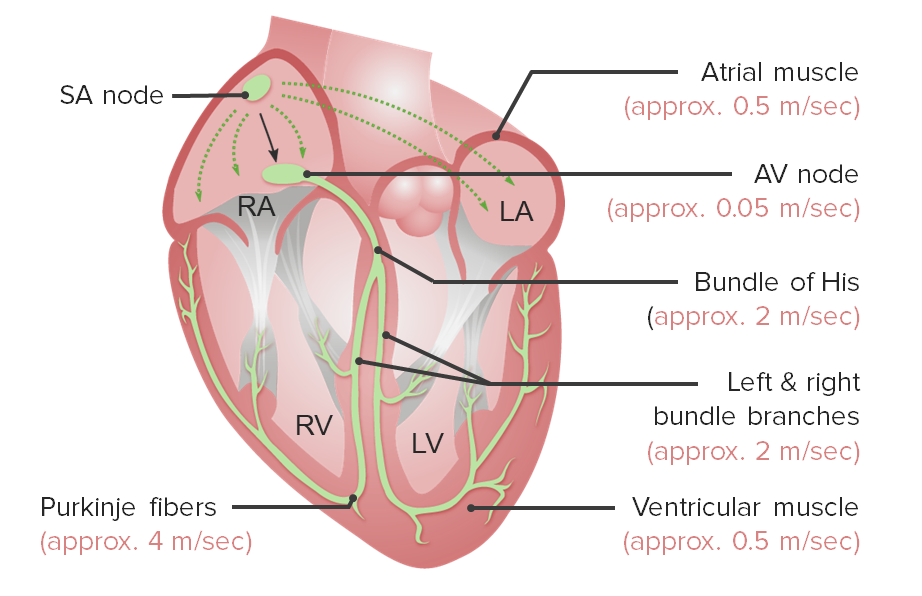
\includegraphics[width=0.8\textwidth]{img/sistemaConduccion.png}
        \caption[Sistema de conducción cardíaca y tiempos de conducción de los respectivos segmentos]{Sistema de conducción cardíaca y tiempos de conducción de los respectivos segmentos\footnotemark}
        \label{fig:sistemaConduccion}
    \end{figure}
    \footnotetext{Localización de las células marcapasos dentro del sistema de conducción del corazón. Imagen tomada de lecturio.com. Fuente: \url{https://goo.su/MSZMxUj}}

    \subsection{Electrocardiograma (ECG)}
    Un electrocardiograma (ECG) es un estudio que registra el voltaje generado por los vectores de despolarización y repolarización de las células cardiacas en relación con el tiempo. El ECG es una herramienta útil para evaluar la función cardíaca y detectar problemas cardíacos. \cite{ECG_Definicion}

    El ECG registra la actividad eléctrica del corazón mediante electrodos colocados en la piel del pecho, los brazos y las piernas. Los electrodos detectan las señales eléctricas generadas por el corazón y las transmiten a un dispositivo que registra la actividad eléctrica en forma de ondas.

    Las ondas del ECG son las siguientes:

    \begin{itemize}
        \item \textbf{Onda P}: Representa la despolarización auricular, es la suma de los vectores de despolarización de ambas aurículas.
        \item \textbf{Intervalo PR}: Representa el tiempo transcurrido desde la despolarización auricular, hasta la despolarización ventricular. Incluye la onda P y el segmento PR. Éste último elemento es una línea isoeléctrica, establecida gracias al retardo fisiológico que sufre la conducción eléctrica en el nodo aurículoventricular. Sin este retraso mencionado, las aurículas y los ventrículos se despolarizarían casi al mismo tiempo, siendo imposible el funcionamiento correcto del corazón para que la sangre pase por sus diferentes cavidades ordenadamente.
        \item \textbf{Onda Q}: Indica el inicio de la despolarización ventricular, específicamente el vector de despolarización septal.
        \item \textbf{Onda R}: Representa el segundo vector de despolarización, correspondiente a la pared libre del ventrículo izquierdo. Es normalmente la onda con mayor voltaje, debido a que el ventrículo izquierdo es el que mayor cantidad de células posee, por ende, la actividad eléctrica es mayor y el vector es más grande.
        \item \textbf{Onda S}: Corresponde al último vector de despolarización ventricular, originado en las bases de los ventrículos.
        \item \textbf{Complejo QRS}: Es la suma de los tres vectores de despolarización anteriores, y juntos representan a la despolarización ventricular.
        \item \textbf{Segmento ST}: Es un periodo de inactividad que separa la despolarización ventricular de la repolarización ventricular, va desde el final del complejo QRS hasta el comienzo de la onda T. 
        \item \textbf{Intervalo QT}: Se extiende desde el comienzo del complejo QRS hasta el final de la onda T y representa la sístole eléctrica ventricular, o lo que es lo mismo, el conjunto de la despolarización y repolarización ventricular. La medida de este intervalo depende de la frecuencia cardiaca, de forma que el intervalo QT se acorta cuando la frecuencia cardiaca es alta, y se alarga cuando la frecuencia cardiaca es baja. Por lo anterior, cuando se mide, es necesario corregirlo de acuerdo con la frecuencia cardíaca utilizando la fórmula de Bazett
        \item \textbf{Onda T}: Es la onda que representa la repolarización ventricular.
        \item \textbf{Onda U}: Es una onda de escaso voltaje que puede o no estar presente en el trazado del electrocardiograma. Se debe a la repolarización de los músculos papilares
        \item \textbf{Intervalo RR}: Es el intervalo que abarca desde una onda R, hasta la onda R de la siguiente despolarización, es decir dos ondas R sucesivas. En un paciente sano, debe permanecer a un ritmo constante. La medida de este intervalo dependerá de la frecuencia cardiaca.
    \end{itemize}

    \begin{figure}[H]
        \centering
        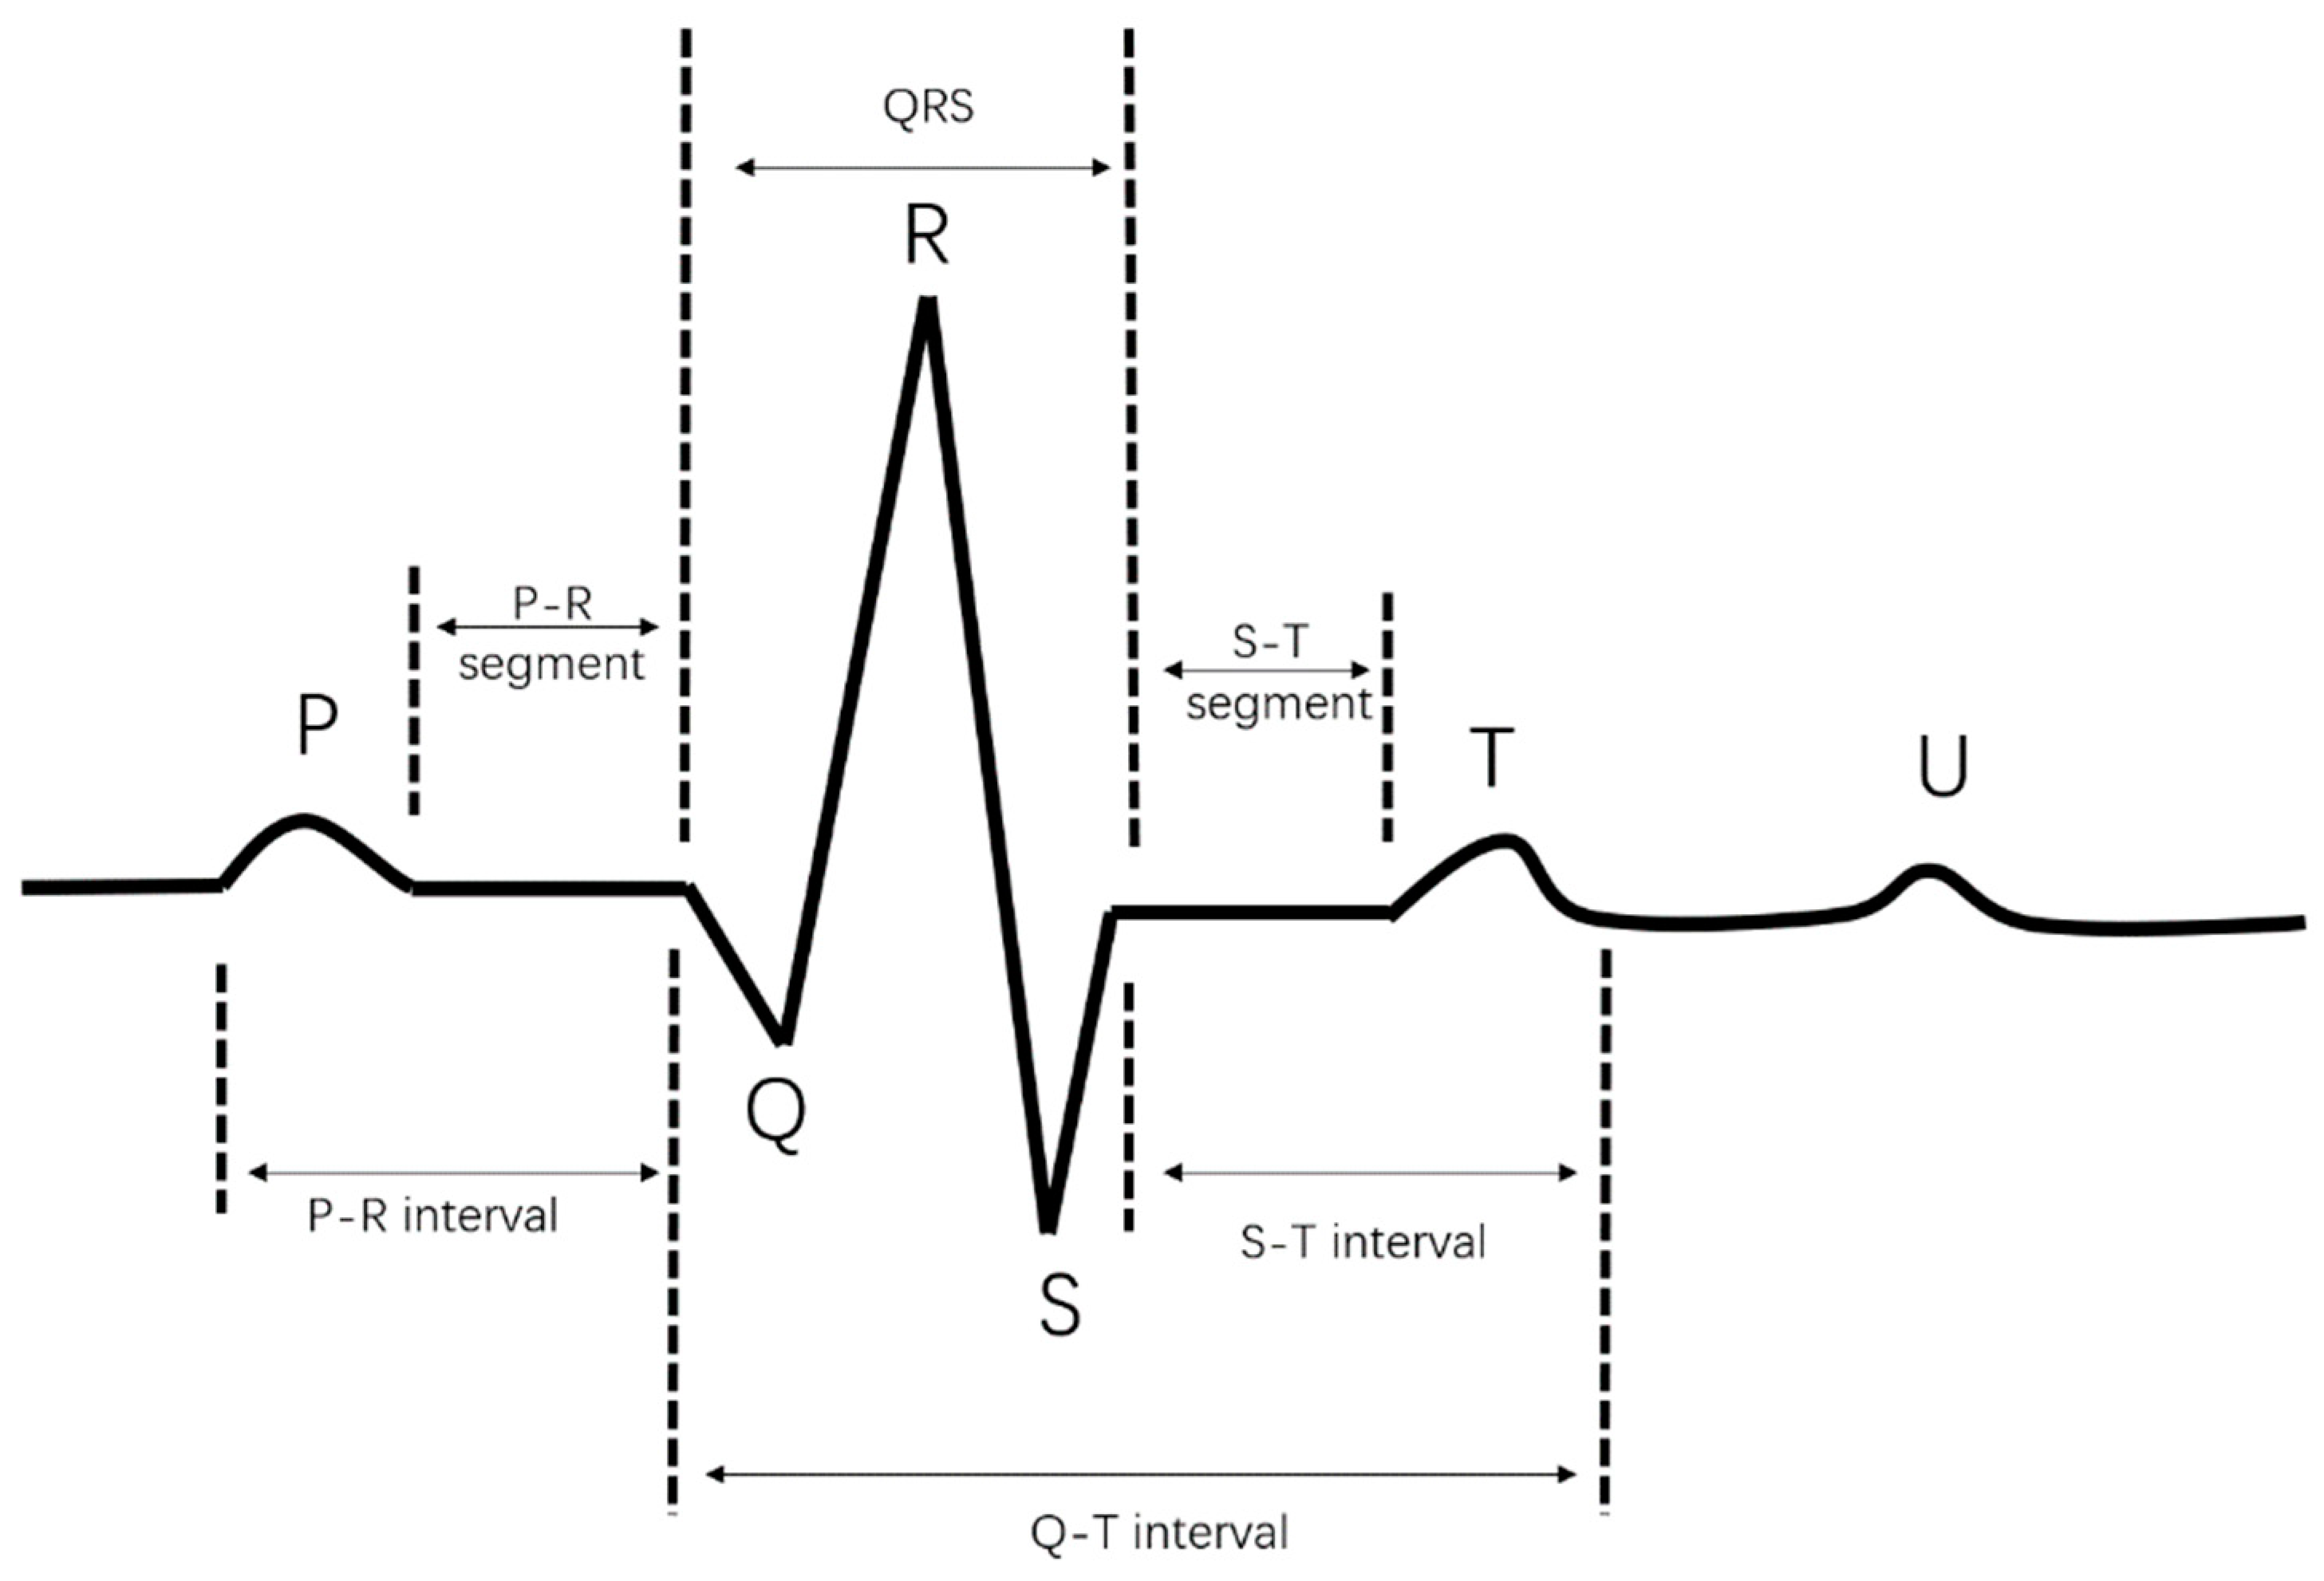
\includegraphics[width=0.8\textwidth]{img/ECG_ondas.png}
        \caption[Ondas de un electrocardiograma]{Ondas de un electrocardiograma\footnotemark}
        \label{fig:ECG_ondas}
    \end{figure}
    \footnotetext{Muestra todas las ondas que conforma un electrocardiograma. Imagen tomada del Departamento de Fisiología de la UNAM. Fuente: \url{https://goo.su/EuR8}}

    \subsection{Presión Arterial}
    La presión arterial es la fuerza que ejerce la sangre contra las paredes de las arterias. La presión arterial se mide en milímetros de mercurio (mmHg) e incluye dos mediciones: la presión sistólica, que se mide durante el latido del corazón (momento de presión máxima), y la presión diastólica, que se mide durante el descanso entre dos latidos (momento de presión mínima) \cite{PresionArterialDefinicion}.

    La presión arterial normal es de 120/80 mmHg, la presión arterial alta (hipertensión) es de 140/90 mmHg o más y la presión arterial baja (hipotensión) es de 90/60 mmHg o menos \cite{DOF}.